%!TEX root = ../../Main.tex
\graphicspath{{Chapters/AssessmentTechniques/}}
%-------------------------------------------------------------------------------

\chapter{Assessment Techniques}

\section{ACR} % (fold)
\label{sec:acr}

Absolute Category Rating

Rating scale: 5, 9 or 11 point system (Bad, Poor, Fair, Good, Excellent)

Images are presented one at a time and rated independently.

Method: Each image is presented for 10 seconds followed by a gray screen from where the observer gets to evaluate the image.

\begin{figure}[H]
	\centering
	
\includegraphics[width = \columnwidth]{Img/ACR}
	\caption{ACR method}
	\label{fig:acrMethod}
\end{figure}

% section acr (end)

\section{DCR} % (fold)
\label{sec:dcr}

Degradation Category Rating

Rating scale: 5 point system (Very annoying, Annoying, Slightly annoying, Perceptible but not annoying, Imperceptible)

Images are presented in pairs and the first stimulus in each pair is always the source reference

Method: The original image is shown for 10 seconds followed by a pause (gray screen) for 2 seconds. The image for evaluation is then shown for 10 seconds followed by a gray screen and the observer has 10 second to evaluate the image. The pair of images can be presented simultaneously. Annex C

\begin{figure}[H]
	\centering
	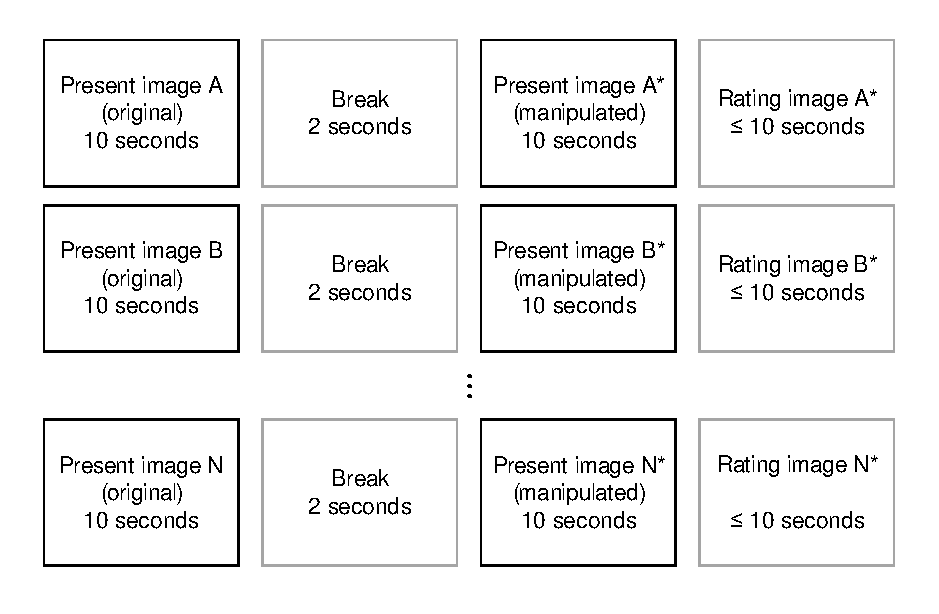
\includegraphics[width = \columnwidth]{Img/DCR}
	\caption{DCR method}
	\label{fig:dcrMethod}
\end{figure}

Comments:
 - Thus, when it is important to check the fidelity with respect to the source signal, DCR method should be used. [ITU]

% section dcr (end)

\section{SAMVIQ} % (fold)
\label{sec:samviq}

Subjective assessment methodology for video quality

Rating scale: 0 - 100 (Bad, Poor, Fair, Good, Excellent)

A 10 or 15 seconds maximum visualization duration of a sequence is sufficient.

Method: The test is carried out scene after scene. Each scene has the known reference, one hidden reference and the number of images to be evaluated. From one scene to another, the sequence access is randomized to prevent the observers from attempting to vote in an identical way according to an established order.

\begin{figure}[H]
	\centering
	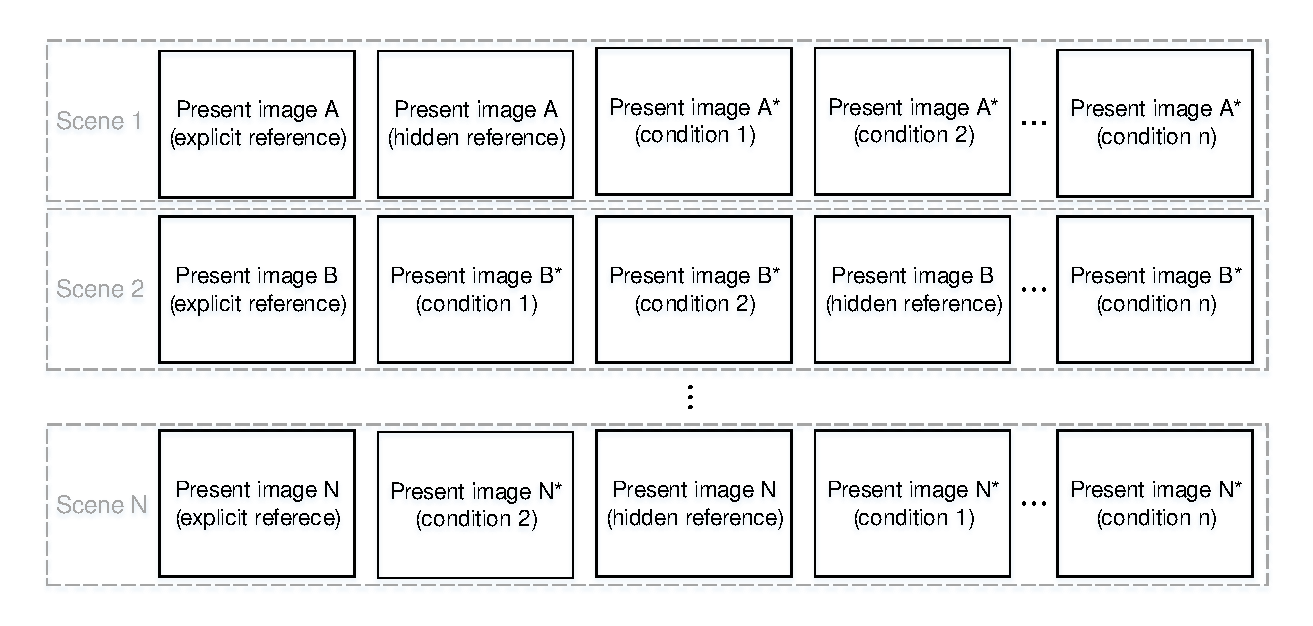
\includegraphics[width = \columnwidth]{Img/SAMVIQ}
	\caption{SAMVIQ method}
	\label{fig:samviqMethod}
\end{figure}

% section samviq (end)